\documentclass{beamer}

\usepackage{color}
\usepackage[
%english
ngerman
]{babel}
\usepackage[ruled,linesnumbered]{algorithm2e}
\usepackage[T1]{fontenc}
\usepackage[%
%	latin1,
	utf8
]{inputenc}
\usepackage{ifthen}
\usepackage{rotating}
\usepackage{graphicx}
\usepackage{listings}
\usepackage{subcaption}

\setbeamertemplate{navigation symbols}{}
%\setbeamertemplate{footline}[page number]
\setbeamertemplate{footline}[frame number]

\title{tcpdump Analyse}
\author{Sebastian Menski}
%\institute{Institute of Computer Science\\University of Potsdam}
\institute{Institut für Informatik\\Universität Potsdam}
\date{19. Mai 2016}

\begin{document}

\frame{\thispagestyle{empty}\titlepage}
\frame{\thispagestyle{empty}\tableofcontents{}}

\newcommand{\mytitle}{}

\newcommand{\mysection}[1]{
\renewcommand{\mytitle}{#1}
\section{#1}
 \frame{\thispagestyle{empty}
 \begin{center}
 \textcolor{beamer@blendedblue}{\LARGE\mytitle}
 \end{center}
 }
}

\newcommand{\myframe}[2][\empty]{
\frame{\frametitle{\mytitle}
  \ifthenelse{\equal{#1}{\empty}}
    {#2}
    {\framesubtitle{#1}#2}
}
}

\newcommand{\mybreakframe}[2][\empty]{
\frame[allowframebreaks]{\frametitle{\mytitle}
  \ifthenelse{\equal{#1}{\empty}}
    {#2}
    {\framesubtitle{#1}#2}
}
}
\newcommand{\myfframe}[2][\empty]{
\frame[fragile]{\frametitle{\mytitle}
  \ifthenelse{\equal{#1}{\empty}}
    {#2}
    {\framesubtitle{#1}#2}
}
}


\mysection{Fragestellung}

\myframe{
  \begin{itemize}
  \item Doktorarbeit von Simon Kiertscher
  \item HTTP Traffic Analyse mit tcpdump
  \item Verliert tcpdump Pakete unter hoher Last?
  \end{itemize}
}

\mysection{tcpdump}

\myframe{
  \begin{itemize}
  \item tcpdump: CLI um Netzwerkpakete aufzuzeichen und zu analysieren
  \item libpcap: Bibliothek um Pakete auf unterschiedlichen Platformen zu filtern
  \item Untersuchte Versionen:
      \begin{itemize}
          \item tcpdump 4.3.0
          \item libpcap 1.3.0
          \item CentOS 5 - Kernel 2.6.18
      \end{itemize}
  \end{itemize}
}

\myframe[Netzwerkstack]{
  \begin{figure}
    \centering
    
\includegraphics[height=0.8\textheight]{images/network-stack}
  \end{figure}
}

\myframe[Linux Socket Filter]{
  \begin{itemize}
      \item Linux Socket Filter (LSF) seit Kernel 2.2
      \item Filter kann an Socket angehangen werden
      \item Berkley Paket Filter (BPF) Programm Assembler ähnlich
      \item Direkter Zugriff auf Paketdaten
  \end{itemize}
}

\myframe[BPF für \texttt{tcpdump -d ip dst host 10.3.9.21 and tcp dst port 80}]{
    \lstinputlisting[numbers=none]{listings/filter.txt}
}

\myframe[Parameter]{
  \begin{itemize}
      \item snaplen (-s): Anzahl der Bytes die von einem Paket aufgezeichnet werden
      \item buffer (-B): Größe des Empfangsbuffers
      \item filter: Socketfilter um Pakete im Kernel zu filtern
  \end{itemize}
}

\mysection{Konzept}

\myframe{
  \begin{itemize}
      \item HTTP Benchmark mit einer hohen Anzahl an Requests
      \item Minimale HTTP Responses
      \item Auswirkung von tcpdump Parametern untersuchen
  \end{itemize}
}

\myframe[Versuchsaufbau]{
  \begin{figure}
    \centering
    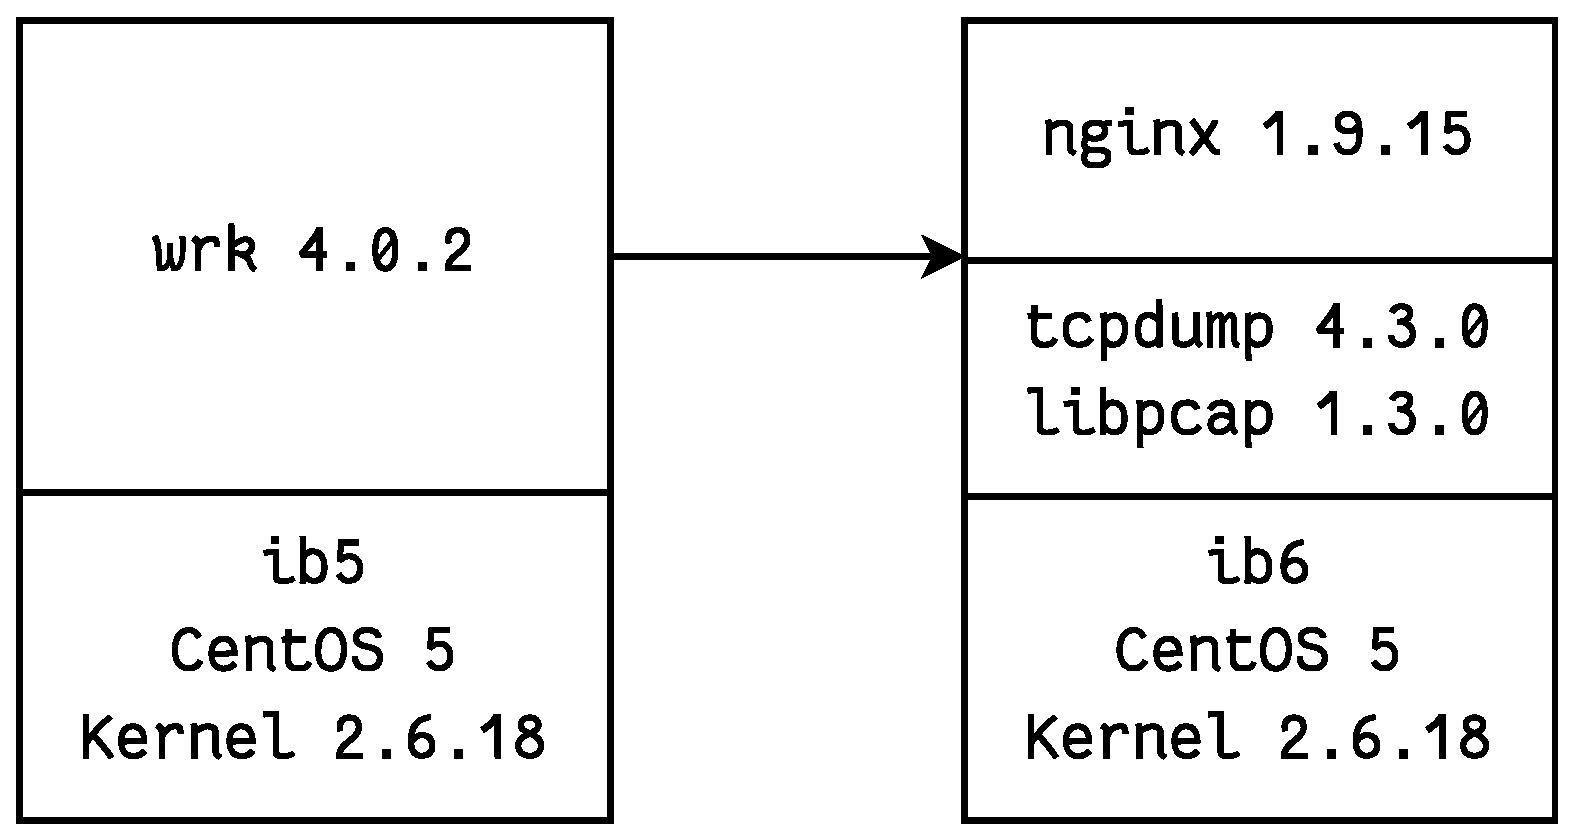
\includegraphics[width=0.8\textwidth]{images/aufbau}
  \end{figure}
}

\myframe[Versuchsaufbau]{
    \begin{itemize}
        \small
        \item wrk -t 4 -c 1024 -d 5m http://ib6
        \item tcpdump -i eth1 -w dump.pcap -s SNAPLEN -B BUFFER FILTER
    \end{itemize}
}

\myframe[nginx Konfiguration]{
    \lstinputlisting[numbers=none,basicstyle=\scriptsize]{listings/nginx.conf}
}


\myframe[Szenarien]{
    \scriptsize
    \begin{table}
      \centering
      \bgroup
      \def\arraystretch{1.3}
      \begin{tabular}{cccp{5.9cm}}
          \textbf{Name} & \textbf{snaplen} & \textbf{buffer} & \textbf{filter} \\\hline\hline
          no & \multicolumn{3}{c}{---} \\\hline
          default & 65535 & 2048 & ip dst host 172.16.0.26 and tcp dst port 80 \\\hline
          snaplen & 142 & 2048 & ip dst host 172.16.0.26 and tcp dst port 80 \\\hline
          buffer  & 65535 & 4096 & ip dst host 172.16.0.26 and tcp dst port 80 \\\hline
          snaplen+buffer & 142 & 4096 & ip dst host 172.16.0.26 and tcp dst port 80 \\\hline
          filter  & 142 & 4096 & ip dst host 172.16.0.26 and tcp dst port 80 and \\
                  & & & 'tcp[((tcp[12:1] \& 0xf0) >> 2):4] = 0x47455420' \\
      \end{tabular}
      \egroup
      \caption{Konfiguration von tcpdump für Messszenarien}
    \end{table}
}

\myframe[Metriken]{
    \begin{itemize}
        \item Anzahl der gesendeten HTTP Requests (wrk)
        \item Anzahl der gefilterten Netzwerkpakete (tcpdump)
        \item Anzahl der verlorenen Netzwerkpakete (tcpdump)
    \end{itemize}
}

\mysection{Messungen}

\myframe{
    \begin{itemize}
        \item Messungen jeweils 5 Minuten und 7 Wiederholungen
        \item Ausgabe von wrk und tcpdump gespeichert
        \item Von allen Metriken wurde er Median genutzt
    \end{itemize}
}

\myframe[wrk Ausgabe]{
    \lstinputlisting[numbers=none,basicstyle=\scriptsize]{listings/wrk.log}
}

\myframe[tcpdump Ausgabe]{
    \lstinputlisting[numbers=none,basicstyle=\scriptsize]{listings/tcpdump.log}
}

\myframe[Ergebnisse]{
\begin{figure}
    \centering
    \includegraphics[width=0.5\textwidth]{images/requests}
    \caption{Anzahl der von wrk gesendeten HTTP Requests}
\end{figure}
}

\myframe[Ergebnisse]{
\begin{figure}
  \begin{subfigure}[b]{0.49\textwidth}
    \includegraphics[width=\textwidth]{images/dropped}
  \end{subfigure}
  %
  \begin{subfigure}[b]{0.49\textwidth}
    \includegraphics[width=\textwidth]{images/dropped-percentage}
  \end{subfigure}
\caption{Paketverlust bevor tcpdump die Pakete auswerten konnte}
\end{figure}
}

\myframe[Ergebnisse]{
\begin{table}
  \scriptsize
  \centering
  \bgroup
  \def\arraystretch{1.2}
  \begin{tabular}{crrrrr}
      & \textbf{Requests} & \textbf{Requests/s} & \textbf{Filtered} & \textbf{Dropped} & \textbf{Dropped \%} \\\hline\hline
no & 120069354 & 400217,48 &  &  & \\\hline
default & 93728797 & 312360,77 & 97520639 & 7446903 & 7,662~\%\\\hline
snaplen & 94144165 & 313743,49 & 97952561 & 1634344 & 1,661~\%\\\hline
buffer & 94197335 & 313920,03 & 98005865 & 1860171 & 1,898~\%\\\hline
snaplen+buffer & 93635020 & 312040,81 & 97422724 & 142459 & 0,145~\%\\\hline
filter & 94126289 & 313676,56 & 94128018 & 3613 & 0,004~\%\\\hline
  \end{tabular}
  \egroup
  \caption{Median der Messwerte für alle Szenarien}
\end{table}
}

\mysection{Zusammenfassung}

\myframe{
\begin{itemize}
    \item Unter hoher Last ist Paketverlust wahrscheinlich
    \item Optimierte Parameter können den Paketverlust reduzieren
    \item Zählen von HTTP Requests ist sehr speziell und optimierbar
    \item tcpdump sollte getrennt von SUT betrieben werden
\end{itemize}
}


\end{document}
